\lstset{language=Python}
\definecolor{light-gray}{gray}{0.9}
\lstset{backgroundcolor=\color{light-gray}}
\lstset{aboveskip=1em,belowskip=1em,showspaces=false,showstringspaces=false}


\if 0

% WEH - For now, let's omit this introduction since it needs to be 
%       reworked anyway.

\SANDsection{Introduction}

% TODO: More references here

Many planning situtations involve the analysis of several objectives
that reflect a hierarchy of decision-makers.  For example, policy
decisions are made at different levels of a government, each of
which has a different objective and decision space.  Similarly, robust planning
against adversaries is often modeled with a 2-level hierarchy, where
the defensive planner makes decisions that account for adversarial
response.

\textit{Multilevel optimization} techniques partition control over
decision variables amongst the levels.  Decisions at each level of
the hierarchy may be constrained by decisions at other levels, and
the objectives for each level may account for decisions made at
other levels.  In practice, multilevel problems have proven difficult
to solve, and most of the literature has focused on \textit{bilevel
programs}, which model a 2-level hierarchy~\citep{ColMarSav07}.

Although multilevel problems arise in many applications, few algebraic
modeling languages (AML) have integrated capabilities for expressing
these problems.  AMLs are high-level programming languages for
describing and solving mathematical problems, particularly
optimization-related problems~\citep{Kal04}.  AMLs provide a mechanism
for defining variables and generating constraints with a concise
mathematical representation, which is essential for large-scale,
real-world problems that involve thousands or millions of constraints
and variables.  GAMS~\citep{GAMS}, YALMIP~\cite{Lof04} and Pyomo
provide explicit support for modeling bilevel programs.  A variety
of other AMLs support the solution of bilevel programs through the
expression of Karush-Kuhn-Tucker conditions and associated
reformulations using mixed-complementarity conditions, but these
reformulations must be expressed by the user in these AMLs.

In this paper, we describe new functionality in Pyomo 4.3 for
expressing and optimizing multilevel models in the Pyomo modeling
environment.  Pyomo is an open-source software package that supports
the definition and solution of optimization applications using the
Python language~\cite{pyomotrac,pyomoweb,HarWatWoo11,HarLaiWatWoo12}.
Python is a powerful programming language that has a clear, readable
syntax and intuitive object orientation.  Pyomo uses an object-oriented
approach for defining models that contain decision variables,
objectives, and constraints.  

The main point of this paper is to demonstrate that Pyomo provides
an intuitive syntax for expressing multilevel optimization problems.
Multilevel models can be easily expressed with Pyomo modeling
components for submodels, which can be nested in a general manner.
Further, Pyomo's object-oriented design naturally supports the
ability to automate the reformulation of multilevel models into
other forms.  In particular, we describe Pyomo's capabilities for
transforming bilevel models for several broad classes of problems.
We describe Pyomo meta-solvers that transform bilevel programs into
mixed integer programs (MIP) or nonlinear programs (NLP), which are
then optimized with standard solvers.

The remainder of this paper is organized as follows.
Section~\ref{sec:problems} describes motivating classes of bilevel
programming problems.  Section~\ref{sec:design} describes how Pyomo
supports modeling of submodels.  Sections~\ref{sec:BLP} and~\ref{sec:QMM}
describe transformations that automate the reformulation of bilevel
programs and meta-solvers in Pyomo that leverage these transformations
to support global and local optimization of bilevel programs.
Section~\ref{sec:discussion} discusses Pyomo's ability to model multilevel problems, and possible extensions for non-cooperative bilevel programs.

\fi


\SANDsection{Expressing Multilevel Programs}
\label{sec:modeling}

In multilevel optimization problems, a subset of decision variables
at each level is constrained to take values associated with an
optimal solution of a distinct, lower level optimization problem.
For example, a general formulation for bilevel programs is
\begin{equation}
\label{eqn:bilevel}
\begin{array}{ll}
\min_{x \in X, y \in Y}   & F(x,y)\\
\st                 & G(x,y) \leq 0\\
                    & y \in P(x)
\end{array}
\end{equation}
where
\[
\begin{array}{llll}
P(x) & = & \argmin_{y \in Y}    & f(x,y)\\
 & &                            & g(x,y) \leq 0.
\end{array}
\]
$P(x)$ defines a \textit{lower-level problem}, which may have multiple solutions.
Here $x$ is the primary upper-level decision, and $y$ is the anticipated lower-level 
decision.

When $P(x)$ contains multiple solutions, this formulation ensures
that the selected value for $y$ will minimize $F(x,y)$.  Consequently,
this formulation has been called \textit{optimistic} or
\textit{cooperative}, since the selection of the lower-level decision
variables minimized the upper-level objective.  Most research on
bilevel programming has considered this problem, since this formulation
has an optimal solution under reasonable assumptions.

Many authors use a more compact form to express (\ref{eqn:bilevel}):
\begin{equation}
\label{eqn:bilevel-compact}
\begin{array}{lll}
\min_{x \in X, y \in Y}   & F(x,y) & \\
\st                       & G(x,y) \leq 0 & \\
                          & \min_{y \in Y}    & f(x,y)\\
                          &                   & g(x,y) \leq 0
\end{array}
\end{equation}
This notation defines an implied constraint by not explicitly referencing the solution to the lower-level problem.

Alternatively, a \textit{pessimistic} bilevel problem is when \eqref{eqn:bilevel} is expressed as 

\begin{equation}
\label{eqn:bilevel_pess}
\begin{array}{lll}
\min_{x \in X}   & F(x)\\
\st                 & G(x,y) \leq 0 &\forall y \in P(x)
\end{array}
\end{equation}
where 
\[
\begin{array}{llll}
P(x) & = & \argmin_{y \in Y}    & f(x,y)\\
 & &                            & g(x,y) \leq 0.
\end{array}
\]
This formulation ensures that the upper-level problem is feasible for all values $y$ including the least favorable outcome of the lower-level problem $P(x)$. 
It is common to see the pessimistic problem written as
\begin{equation}
\label{eqn:bilevel_pess_minmax}
\min_{x \in X}\max_{y \in P(x)} H(x,y).
\end{equation}
Though formulation (\ref{eqn:bilevel_pess_minmax}) makes clear the selected value for $y$ will in fact maximize $H(x,y)$, note that it is actually less general than (\ref{eqn:bilevel_pess}) since we can rewrite it in the form of (\ref{eqn:bilevel_pess}), as
\[
\begin{array}{lll}
\min_{x, \tau} &\tau \\
\st & \tau \geq H(x, y) & \forall y \in P(x) \\
& x \in X,
\end{array}
\]
but it is not always possible to tranform problems in the form of (\ref{eqn:bilevel_pess_minmax}) to (\ref{eqn:bilevel_pess}) without definting functions $H(x,y)$ and $f(x,y)$ on the extended real line \cite{WiesemannTKR2013}.
Unless otherwise stated, the canonical bilevel problem in the subsequent examples will be derived from the \textit{optimistic} approach presented in \eqref{eqn:bilevel}.


\subsection{Introduction to \code{pao}}

The Python package \code{pao} is a bilevel mathematical programming library that has dependencies on \code{pyomo} for syntactical representation of bilevel problems. Similar to \code{pyomo} mathematical problems, \code{pao} problems can be optimized with solvers that are written either in Python or in compiled, low-level languages.

The \code{pao} package uses the \code{SubModel} component in \code{pyomo} to declare a block that defines a lower-level problem. 
For example, consider the bilevel problem:
\begin{equation}
\label{eqn:bilevel_ex1}
\begin{array}{ll}
\min_{v \in [1,2], x \in [1,2]}   & v + x + y\\
\st                 & v + x\geq 1.5\\
                    & y \in P(v,x)
\end{array}
\end{equation}
where 
\[
\begin{array}{llll}
P(v,x) & = & \argmin_{w \in [-1,1], y \in [1,2]}    & x + w\\
 & &                            &  y + w \leq 2.5
\end{array}
\]
which can be represented in \code{pao} as:

\begin{qlisting}
model = ConcreteModel()
model.x = Var(bounds=(1,2))
model.v = Var(bounds=(1,2))
model.sub = SubModel()
model.sub.y = Var(bounds=(1,2))
model.sub.w = Var(bounds=(-1,1))

model.o = Objective(expr=model.x + model.sub.y + model.v, sense=minimize)
model.c = Constraint(expr=model.x + model.v >= 1.5)
model.sub.o = Objective(expr=model.x+model.sub.w, sense=maximize)
model.sub.c = Constraint(expr=model.sub.y + model.sub.w <= 2.5)
\end{qlisting}
This Pyomo model defines four variables,  \code{v}, \code{x}, \code{sub.w} and \code{sub.y}.
Variables \code{v}  and \code{x} are declared in the upper-level
problem, and \code{v} only appears in the upper-level problem.
Variables \code{sub.w} and \code{sub.y} are declared in the submodel.
However, note that the \code{sub.y} variable appears in the upper-level
problem, while the \code{sub.w} variable only appears in the
lower-level problem.

While this syntax mimics the abstract structure of \eqref{eqn:bilevel-compact} -- as represented directly in \eqref{eqn:bilevel_ex1} --  it adds additional abstractions that make it difficult to interpret:
\begin{itemize}

\item It can be difficult to easily discern which are the upper and lower level variables.  In general, Pyomo does not place strong restrictions on the location of variable declarations relative to the location where those variables are used in expressions.  Thus, while a hierarchical block structure suggests nested model representations, this is not strongly enforced when objective and constraint expressions are generated.\\
\mbox{}\\
IDEA: Enforce a stronger semantics on PAO block representations for bilevel programs.\\
IDEA: Use model annotations to denote upper- and lower- level variables.\\

\item This syntax does not indicate how the solution of the lower level relates to constraints in the upper level problem.  Specifically, there is no explicit indication how solutions to the lower level problem relate to variables in the upper-level problem.  In simple applications, where there is a direct correspondence of variables (using the same names), this simple syntax may be sufficient.  But in more complex applications the variables need not have the same naming in the upper- and lower-level problems.  Thus, PAO needs a mechanism to associate these variables.

\end{itemize}

There are also practical issues that reflect the needs of users with
respect to the solution of bilevel programs.  Generally, it is assumed
that the solution of~(\ref{eqn:bilevel}) consists of the optimal upper-
and lower-level variables.  However in practice a user may only need
the optimal upper-level variables.  If true, this may allow for a
faster response.  Additionally, there's another solution response that
may be of interest to analysts, where solution consists of the optimal
upper-level variables along with other diagnostic information related
to the solution of the lower-level problem.  For example, in some cases
the dual of the lower-level problem can be used, so the solution to the
problem could include the dual lower-level variables.  Note that these
considerations also generalize to multi-level problems, where a user may
wish to specify the requirements for a solution value (e.g. needing only
the first- and second-level variables in a tri-level problem).

The following subsections describe ideas for expressing and solving multi-level programs, with the
goal of defining some alternatives that the PAO developers can discuss while refining the 
problem representations in PAO.

\subsection{Using Set Notation}

IDEA: Declare the SubModel using arguments that define the lower-level variables whose
optimal value constrains the upper-level variables.

\begin{qlisting}
model = ConcreteModel()

model.x = Var(bounds=(1,2))
model.v = Var(bounds=(1,2))
model.y = Var(bounds=(1,2))

model.o = Objective(expr=model.x + model.v + model.y)
model.c = Constraint(expr=model.x + model.v >= 1.5)

model.sub = SubModel(fixed=[model.x, model.v], y=model.y)

# NOTE - model.sub.y is implicitly defined
model.sub.w = Var(bounds=(-1,1))

model.sub.o = Objective(expr=model.x + model.sub.w, sense=maximize)
model.sub.c = Constraint(expr=model.sub.y + model.sub.w <= 2.5)
\end{qlisting}
QUESTION: Is the last line correct here???\\

\noindent PROS
\begin{itemize}
\item More explicit than pyomo.bilevel
\end{itemize}
CONS
\begin{itemize}
\item Users may not appreciate this difference and use model.y instead of model.sub.y.  Can we robustly catch errors when that happens?
\item May not be able to capture complex relationships between upper- and lower-level variables
\item May not be useful for defining pessimistic relationships.
\end{itemize}


\subsection{Using Set Notation}

IDEA:  What if the SubModel declaration defined a set, which can be explicitly used to
define a constraint (similar to~(\ref{eqn:bilevel})?

TODO ...


\subsection{Using New Pyomo Notation}

For example, consider the bilevel problem:
\begin{equation}
\label{eqn:bilevel_ex1}
\begin{array}{ll}
\min_{v \in [1,2], x \in [1,2]}   & v + x + y\\
\st                 & v + x\geq 1.5\\
                    & y \in P(v,x)
\end{array}
\end{equation}
where 
\[
\begin{array}{llll}
P(v,x) & = & \argmin_{w \in [-1,1], y \in [1,2]}    & x + w\\
 & &                            &  y + w \leq 2.5
\end{array}
\]
which can be represented in \code{pao} pseudo-code as:

\begin{qlisting}
from pyomo.environ import *
from pao.bilevel import *
model = ConcreteModel()
model.x = Var(bounds=(1,2))
model.v = Var(bounds=(1,2))
model.y = Var(bounds=(1,2))
model.w = Var(bounds=(-1,1))
model.upper = SubModel(vars=[model.x,model.v])
model.lower = SubModel(vars = [model.y,model.w], parent = upper, 
		type = optimistic, argmin = model.y)

model.upper = Objective(expr=model.x + model.y + model.v, sense=minimize)

model.o = Objective(expr=model.x + model.y + model.v, sense=minimize)
model.c = Constraint(expr=model.x + model.v >= 1.5)
model.lower.o = Objective(expr=model.x+model.w, sense=maximize)
model.lower.c = Constraint(expr=model.y + model.w <= 2.5)
\end{qlisting}

\noindent PROS
\begin{itemize}
\item Requiring that each level of the problem be defined in a SubModel() block, which enables each submodel to be solved independently
\item The user must specify important aspects about that level of the problem when instantiating the SubModel()
\end{itemize}
CONS
\begin{itemize}
\item Implicitly fixes the vars not specified in the vars argument to the SubModel() to their current value
\item Variables have to be defined prior to instantiating the submodel; the user may want to define these on the SubModel() block
\end{itemize}

\SANDsection{Special Cases}
\label{sec:problems}

The following subsections describe specializations of
Equation~(\ref{eqn:bilevel}) that will be explored in greater detail
throughout this paper.  These are well-studied classes of bilevel
programs that that can be reformulated into other canonical
optimization forms.


\subsection{Linear Bilevel Programs with Continuous Variables}

Multilevel linear programming considers the case where decision
variables are continuous, and both objectives and contraints are
linear.  In the 2-level case, we have the following linear bilevel program:
\begin{equation}
\label{eqn:bilevel_A}
\begin{array}{lll}
\min_{x, y}         & c^T_1 x + d^T_1 y & \\
\st                 & A_1 x + B_1 y \leq b_1 & \\
                    & x \geq 0 & \\
                    & \min_{y}  & c^T_2 x + d^T_2 y\\
                    &           & A_2 x + B_2 y \leq b_2\\
                    &           & y \geq 0
\end{array}
\end{equation}


\subsection{Quadratic Min/Max}

Consider the case where the lower-level decisions $y$ do not constrain the upper-level decisions.  Let
\[
X = \{ x \mid A_1 x \leq b, x \geq 0\}
\]
Then we have
\begin{equation}
\label{eqn:bilevel_B}
\begin{array}{lll}
\min_{x \in X} & \max_{y \geq 0} & c^T_1 x + d^T_1 y + x^T Q y\\
& & A_2 x + B_2 y \leq b_2
\end{array}
\end{equation}
In our discussion below, we allow the $x_i$ to be binary without loss of generality.



\SANDsection{Modeling Bilevel Programs}
\label{sec:design}


\subsection{Pyomo Models}

Pyomo supports an object-oriented design for the definition of
optimization models.  The basic steps of a simple modeling process are as follows:
\begin{quote}
\begin{enumerate}
\item Create model object and declare components
\item Instantiate the model
\item Apply solver
\item Interrogate solver results
\end{enumerate}
\end{quote}
In practice, these steps may be applied repeatedly with different
data or with different constraints applied to the model.  However,
we focus on this simple modeling process throughout this paper.

A Pyomo {\em model} consists of a collection of modeling {\em
components} that define different aspects of the model.  Pyomo
includes the modeling components that are commonly supported by
modern AMLs:  components for decision variables, objectives and
constraints are used to express the model, and components for index
sets and symbolic parameters are used to manage data used in model
expressions.  These modeling components are defined in Pyomo through
the following Python classes:
\begin{center}
\begin{tabular}{ll}
\code{Var} & decision variables in a model\\
\code{Objective} & expressions that are minimized or maximized in a model\\
\code{Constraint} \hspace{0.2in} & constraint expressions in a model\\
\code{Set} & set data that is used to define a model instance\\
\code{Param} & parameter data that is used to define a model instance
\end{tabular}
\end{center}\mbox{}

Modeling components are directly added to a Pyomo model object as an attribute of the object.
For example:
\begin{qlisting}
model = ConcreteModel()
model.x = Var()
\end{qlisting}
Pyomo defines two model classes: \code{ConcreteModel} and \code{AbstractModel}.  
In concrete models, components are immediately initialized when
they are added to the model.  In abstract models, components are
explicitly initialized later, which allows the creation of multiple
model instances from a single abstract model.

Another Pyomo component is the \code{Block} class, which defines a
named collection of model components.  Blocks provide a convenient
mechanism for segregating different elements of a model within
separate namespaces, and they can be used to define repetitive model
structure in a concise manner.  For example, the following model
defines two variables \code{x}:
\begin{qlisting}
model = ConcreteModel()
model.x = Var()
model.b = Block()
model.b.x = Var()
\end{qlisting}
Block \code{b} defines a namespace that allows these two variables to be
uniquely referenced.

\subsection{Modeling Bilevel Programs}

The \code{pyomo.bilevel} package extends Pyomo by defining a new
modeling component: \code{SubModel}.  The \code{SubModel} component
defines a subproblem that represents the lower level decisions in
a bilevel program.  This component is like a \code{Block} component;
any components can be added to a \code{SubModel} object.  In general,
a submodel is expected to have an objective, one or more variables
and it may define constraints.

The \code{SubModel} class generalizes the \code{Block} component
by including constructor arguments that denote which variables in
the submodel should be considered fixed or variable.  When expressions
in a submodel refer to variables defined outside of the submodel,
the user needs to indicate whether these are fixed values defined
by an upper-level problem.  Fixed variables are treated as constants
within the submodel, but non-fixed variables are defined by the
current submodel or by a lower-level problem.

Consider the following example:
\begin{equation}
\begin{array}{lll}
\min_{x, y, v}      & x + y + v & \\
\st                 & x + v \geq 1.5 \\
                    & 1 \leq x \leq 2 &\\
                    & 1 \leq v \leq 2 & \\
                    & \max_{y,w}  & x + w\\
                    &           & y + w \leq 2.5 \\
                    &           & 1 \leq y \leq 2\\
                    &           & 1 \leq w \leq 2
\end{array}
\end{equation}

\newpage
The following Pyomo model defines four variables, \code{x}, \code{v}, \code{sub.y} and \code{sub.w}:
\listing{examples/simple.py}{pyomo}{2}{15}
Variables \code{x} and \code{v} are declared in the upper-level
problem, and \code{v} only appears in the upper-level problem.
Variables \code{sub.y} and \code{sub.w} are declared in the submodel.
However, note that the \code{sub.y} variable appears in the upper-level
problem, while the \code{sub.w} variable only appears in the
lower-level problem.

\if 0
 {examples/simple_implicit.py}{pyomo}{2}{16}
The submodel object declares that the \code{x} variable is fixed,
so it is treated as an upper-level variable.  
\fi

These modeling capabilities are quite general.  Expressions in
submodels can be linear or nonlinear, convex or nonconvex, continuous
or discontinuous, and more.  Additionally, submodels can be nested
to an arbitrary degree.  Thus, the range of bilevel programs that
can be expressed with Pyomo is quite broad.  However, the real
challenge is solving these models.  The following sections describe
two general strategies for solving the two classes of bilevel
programs described in Section~\ref{sec:problems}.

In each section we describe model transformations and their use in
meta-solvers.  Pyomo's object-oriented design supports the structured
transformation of models.  Pyomo can iterate through model components
as well as nested model blocks.  Thus, model components can be
easily transformed locally, and global data can be collected to
support global transformations.  Further, Pyomo components and
blocks can be activated and deactivated, which facilitates \textit{in
place} transformations that do not require the creation of a separate
copy of the original model.



\if 0
Similarly, the submodel could have been declared as:
\begin{qlisting}
model.sub = SubModel(var=model.y)
\end{qlisting}
The \code{fixed} and \code{var} arguments complement each other,
and they will likely be used in different contexts.
\fi


\if 0
\subsection{Comparison with GAMS}
\label{gams}

To our knowledge, GAMS is the only modern algebraic modeling language
(AML) that supports the definition and automated analysis of bilevel
programs.  Thus, it is worth comparing Pyomo's bilevel modeling
capability with GAMS; we later contrast the solution strategies
supported by GAMS and Pyomo.

Consider the following bilevel program described by Bard~\cite{Bard98} (example 5.1.1):
\begin{equation*}
\begin{array}{lll}
\min_{x \geq 0} & x - 4 y & \\
\st & \min_{y \geq 0} & y\\
 & \st & -x -y \leq -3\\
& & -2 x + y \leq 0\\
& & 2 x + y \leq 12\\
& & 3 x - 2 y \leq 4
\end{array}
\end{equation*}

\if 0
The following GAMS model defines a bilevel program for this
model:\footnote{ This is the \code{bard511.gms} model from the
online GAMS EMPLIB.}
\listing{bard511.gms}
GAMS allows modelers to declare equations and inequalities, which
can subsequently be composed into a model.  The \code{emp} solver
exploits this flexibility through its use of a configuration file,
\code{emp.info}, that defines the structure of the bilevel program.
In this example, the \code{emp.info} file is generated automatically, and the equations
\code{defin}, \code{e1}, \code{e2}, \code{e3} and \code{e4} are included in the
submodel.
\fi

The following Pyomo model defines a bilevel program for this model:
\listing{examples/bard511.py}{}{1}{19}
This model defines the bilevel structure in an object-oriented
manner.  Consequently, the structure is an inherent part of the
model, thereby avoiding the use of auxilliary files in the specification of
the model.

Note that the Pyomo example does not describe how the model is
optimized.  The following section describes a specific model
reformulations strategy for a broad class of bilevel programs.
Further, this section describes a generic solver strategy that leverages
this reformulation to provide an automated solution process.
\fi


\SANDsection{Solving Linear Bilevel Programs}
\label{sec:BLP}

We consider the formulation for linear bilevel programs described
in Equation~(\ref{eqn:bilevel_A}):
\begin{equation}
\begin{array}{lll}
\min_{x, y}         & c^T_1 x + d^T_1 y & \\
\st                 & A_1 x + B_1 y \leq b_1 & \\
                    & x \geq 0 & \\
                    & \min_{y}  & c^T_2 x + d^T_2 y\\
                    &           & A_2 x + B_2 y \leq b_2\\
                    &           & y \geq 0
\end{array}
\tag{\ref{eqn:bilevel_A}}
\end{equation}
Following \citet{Bard98}, we can
replace the lower-level problem with corresponding optimality
conditions.  This transformation gives the following model:
\begin{equation}
\label{eqn:bilevel_A_xfrm}
\begin{array}{ll}
\min & c^T_1 x + d^T_1 y\\
\st  & A_1 x + B_1 y \leq b_1\\
     & d_2 + B^T_2 u - v = 0\\
     & b_2 - A_2 x - B_2 y \geq 0 \perp u \geq 0\\
     & y \geq 0 \perp v \geq 0\\
     & x \geq 0, y \geq 0
\end{array}
\end{equation}
This transformation results in a mathematical program with equillibrium constraints (MPEC).

Pyomo's \texttt{pyomo.bilevel} package automates the application
of this model transformation.  For example, if \code{model} defines
an linear bilevel program,  then the code applies this transformation
to change the model in place:
\listing{examples/ex2.py}{transform}{6}{7}
The \code{bilevel.linear\_mpec} transformation modifies the model
by creating a new block of variables and constraints for the
optimality conditions in the lower-level problem.

A variety of solution strategies can leverage this transformation
to support optimization.  Pyomo defines two meta-solvers, which
apply the \code{bilevel.linear\_mpec} transformation and then perform
optimization with a third-party solver.

Consider the following problem, which is Example 5.1.1. in Bard~\citep{Bard98}:
\begin{equation}
\begin{array}{llrrrrrr}
\min_{x, y}     & x - 4 y & &&&&\\
                & x \geq 0 & &&&&\\
\st             & \min_{y} y & &&&&\\
                & \st   & - x &- &y &\leq &-3\\
                &       & -2 x &+ &y &\leq &0\\
                &       & 2 x &+ &y &\leq &12\\
                &       & 3 x &- &2 y &\leq &4
\end{array}
\end{equation}
Note that the last constraint in this example is negated from the text in \citet{Bard98};  this corrects an error in the example, which is reflected in Bard's discussion of the solution to this example.  The Pyomo model for this problem is:
\listing{examples/bard511.py}{}{1}{19}


\subsection{Global Optimization}

Following Fortuny-amat and McCarl~\cite{ForMcC81}, Pyomo's
\code{bilevel\_blp\_global} meta-solver chains together reformulations
to generate the following sequence of models:
\[
\textrm{BLP} \Rightarrow \textrm{MPEC} \Rightarrow \textrm{GDP} \Rightarrow \textrm{MIP},
\]
where GDP refers to generalized disjunctive programs.  Note that
this leverages advanced modeling capabilities in Pyomo for
MPEC~\cite{PyomoMPEC} and GDP~\cite{PyomoGDP}.

Pyomo provides general support for solving MIPs with commercial and
open-source solvers.  The \code{bilevel\_blp\_global} meta-solver
applies these transformations, solves the resulting MIP, and
translates the MIP solution back into the original linear bilevel
program.  The result is a globally optimal solution.  For example,
the \code{pyomo} command can be used to execute the
\code{mpec\_blp\_global} solver using a specified MIP solver:
\datalisting{examples/mip1a.sh}{pyomo}{4}{5}
Note that a ``Big-M'' transformation is used to convert the GDP
model into a MIP.  The default M value is very large, which may
make it difficult to solve the resulting MIP problem.  Hence, this solver includes
a \code{bigM} option that can be used to specify a problem-specific value:
\datalisting{examples/mip2a.sh}{pyomo}{4}{5}

\subsection{Local Optimization}

Pyomo's \code{bilevel\_blp\_local} meta-solver chains together reformulations to generate the
following sequence of models:
\[
\textrm{BLP} \Rightarrow \textrm{MPEC} \Rightarrow \textrm{NLP}.
\]
This leverages model transformations in \code{pyomo.gdp} to transform an MPEC into an NLP through a simple nonlinear transformation adapted from \citet{FerDirMee05}.  For example, the complementarity condition
\[
y \geq 0 \perp w \geq 0
\]
is transformed to the constraints
\[
\begin{array}{l}
y \geq 0\\
w \geq 0\\
y w \leq \epsilon .
\end{array}
\]

Pyomo provides general support for solving NLPs with commercial and
open-source solvers.  The \code{bilevel\_blp\_local} meta-solver
applies these transformations, solves the resulting NLP, and
translates the solution back into the original linear bilevel
program.  In general, the result is a locally optimal solution.
For example, the \code{pyomo} command can be used to execute the
\code{mpec\_blp\_local} solver using a specified NLP solver:
\datalisting{examples/nlp1a.sh}{pyomo}{4}{5}
Note that the tolerance value $\epsilon$ is initially set to a small
value, which some solvers may have difficulty with.  This value can
be explicitly set with the \code{mpec\_bound} option:
\datalisting{examples/nlp2a.sh}{pyomo}{4}{5}



\SANDsection{Solving Quadratic Min-Max Bilevel Programs}
\label{sec:QMM}

We consider the formulation for quadratic min-max bilevel programs
described in Equation~(\ref{eqn:bilevel_B}):
\begin{equation}
\begin{array}{lll}
\min_{x \in X} & \max_{y \geq 0} & c^T_1 x + d^T_1 y + x^T Q y\\
& & A_2 x + B_2 y \leq b_2
\end{array}
\tag{\ref{eqn:bilevel_B}}
\end{equation}
where
\[
X = \{ x \mid A_1 x \leq b, x \geq 0\}.
\]
The lower-level problem
is linear, so we can replace the lower-level problem with corresponding
optimality conditions.  Since, the objectives are opposite and the
upper-level constraints do not constrain the lower level decisions,
we get a single minimization problem.  This transformation gives
the following model:
\begin{equation}
\label{eqn:bilevel_B_xfrm}
\begin{array}{ll}
\min & c^T_1 x + (b_2 - A_2 x)^T \nu\\
\st  & B^T_2 \nu \geq d_1 + Q^T x\\
     & A_1 x \leq b_1\\
     & x \geq 0, \nu \geq 0
\end{array}
\end{equation}
In Pyomo, this is implemented as the \code{bilevel.linear\_dual} transformation.

If $A_2 \equiv 0$, then the lower-level problem does
not constrain the upper-level decisions.  This is a simple case, where the transformation
generates a linear program if the upper-level decision variables
$x$ are continuous and a MIP if some or all of the $x$ are binary.

More generally, suppose that the upper-level decision variables $x$ are
binary and $A_2 \not \equiv 0$.  We can linearize the quadratic terms
in the objective using \code{gdp.bilinear} transformation, which
creates the following disjunctive representation:
\begin{equation}
\begin{array}{ll}
\min & c^T_1 x + b^T_2 \nu - 1^T z\\
\st  & B^T_2 \nu \geq d_1 + Q^T x\\
     & A_1 x \leq b_1\\
     & \left(\begin{array}{l}
       x_i = 0\\
       z_i = 0
       \end{array}\right) \wedge \left(\begin{array}{l}
       x_i = 1\\
       z_i = A^T_2(*,i) \nu
       \end{array}\right)\\
     & x_i \geq \{0,1\},  \nu \geq 0
\end{array}
\end{equation}
Subsequently, this GDP can be transformed into a MIP using a Big-M transformation.

Consider the following network interdiction problem, for which an
attacker eliminates links in a network to minimize the maximum flow
through the network from a fixed source $s$ to a fixed destination
$t$.  Let $N$ be the nodes in the network through which flow occurs.
Let $y_{ij}$ be a variable that indicates flow from node $i$
to node $j$, and let $c_{ij}$ be the maximum capacity on that arc.  The attacker selects 
$b$ variables $x_{ij}$; if $x_{ij}$ is one then the arc is removed.  This network interdiction problem can be
written as:
\begin{equation}
\begin{array}{lllll}
\min_{x \in X} & \max_{y} & \eta & & \\
    & & \sum_{i \in N} y_{in} = \sum_{j \in N} y_{nj} & \forall n \in N & \textrm{(flow balance constraint)}\\
    & & \eta \leq \sum_{j \in N} y_{sj} & & \textrm{(node s flow)}\\
    & & \eta \leq \sum_{i \in N} y_{it} & & \textrm{(node t flow)}\\
    & & 0 \leq y_{ij} \leq t_{ij} (1-x_{ij}) & \forall \;\textrm{arcs}\; (i,j) & \textrm{(capacity constraint)}
\end{array}
\end{equation}
where
\[
X = \left\{x \mid x_{ij} \in \{0,1\}, \sum_{i,j} x_{ij} \leq b\right\}.
\]

\newpage
The following Pyomo model describes this bilevel program:
\datalisting{examples/interdiction.py}{}{1}{42}
In this example, the file \code{interdiction\_data.py} defines a
simple network with 6 nodes (including $s$ and $t$), adapted from
an example by Will Traves:
\begin{center}
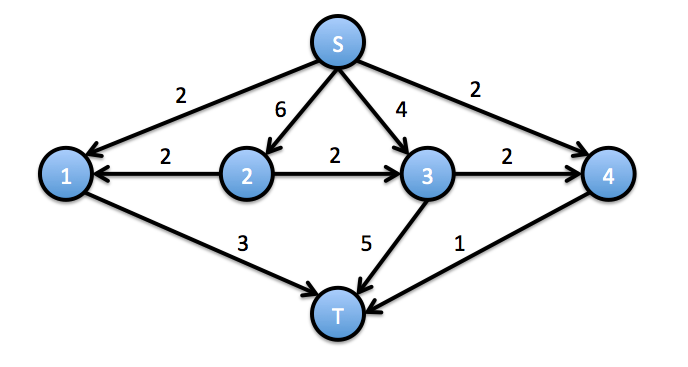
\includegraphics[scale=0.4]{network.png}
\end{center}

Pyomo's \code{bilevel\_ld} meta-solver applies the
\code{bilevel.linear\_dual} transformation and then applies subsequent
transformations when $A_2 \not \equiv 0$.
\datalisting{examples/ld1a.sh}{pyomo}{4}{5}
Note that this solver includes a \code{bigM} option that can be
used to specify a problem-specific value when a MIP is generated
from a GDP.



\SANDsection{Discussion}
\label{sec:discussion}

Note that Pyomo's ability to model multilevel optimization problem
extends far beyond the bilevel programs that are currently supported.
For example, declarations of \code{SubModel} can be arbitrarily
nested with clear semantics.  For example, consider the following trilevel model~\cite{ZhaLuMonZen10}:
\[
\begin{array}{ll}
\min_{x, y, z}  & x - 4y + 2z\\
\st             & -x -y \leq -3\\
                & -3x +2y -z \geq -10\\
                & \begin{array}{ll}\\
                    \min_{y,z} & x + y - z\\
                    \st & -2x + y -2z \leq -1\\
                        & 2x + y + 4z \leq 14\\
                        & \begin{array}{ll}\\
                            \min_{z} & x - 2y - 2z\\
                            \st & 2x - y - z \leq 2
                          \end{array}
                    \end{array}
\end{array}
\]
The following model illustrates how this trilevel model could be implemented in Pyomo:
\listing{examples/trilevel.py}{pyomo}{2}{21}

Pyomo use of object-oriented model specification makes it fundamentally
different from the specification of bilevel models in GAMS and
YALMIP.  Both GAMS and YALMIP allow users to specify expressions
for variables, objectives and constraints, and then the users
specifies which of these are associated with an upper-level or
lower-level problem.  This design allows users to mix-and-match
different modeling components in a flexible manner.  However, it
is limited to a strictly bilevel form.  By contrast, Pyomo submodels
can be nested in an arbitrary manner.  This includes multilevel
models, as was just illustrated.  But it also allows for the
specification of a tree of nested submodels.  For example, Pyomo
supports the specification of independent submodels at the same
level, which can be used to model a single agent cooperating with
decisions for two independent agents that make subsequent decisions..

Earlier, we noted that Pyomo supports optimistic or cooperative
bilevel models.  It seems relatively straightforward to extend
Pyomo's current semantics to support pessimistic bilevel models.
For example, a \code{pessimistic} constructor option could be added
to the \code{SubModel} component.  This capability will be added
when transformations and/or solvers are added to Pyomo for these
bilevel models.
